\begin{frame}
	\frametitle{Lithosphäre - Gestein}

	\begin{figure}
		\centering
		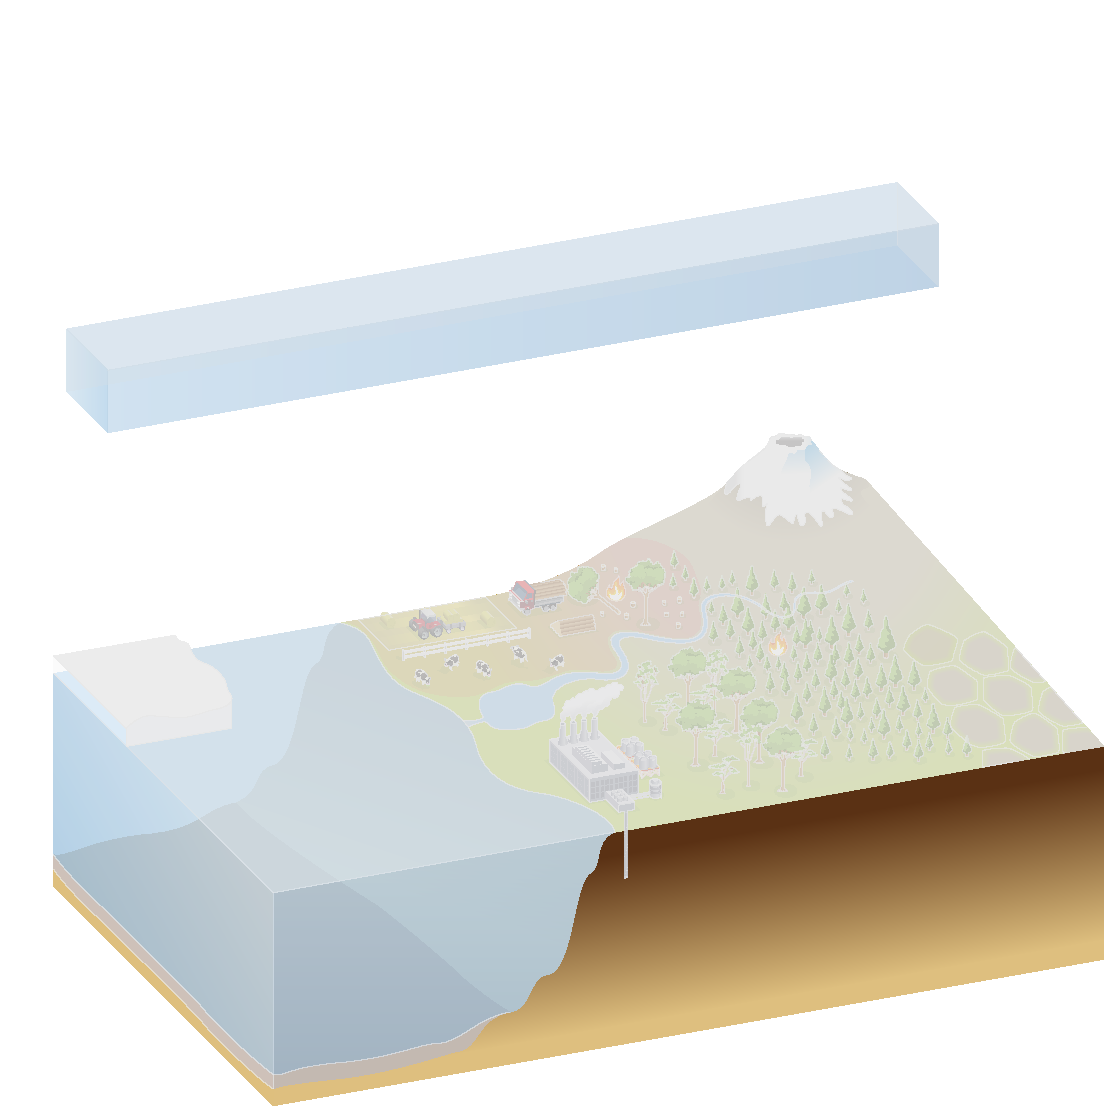
\includegraphics[trim={1cm 0cm 0cm 3cm}, clip, width=0.55\linewidth]{%
        bilder/climate_components/global_climate_components_lithosphere.pdf}
		\caption{Die Lithosphäre besteht aus der Erdkruste und dem relativ starren Teil des oberen Erdmantels.}
	\end{figure}

	\note{
		\begin{itemize}
			\item[] Die Lithosphäre ist die äußerste Schicht des Erdkörpers. Sie besteht aus der Erdkruste und dem äußersten Teil des Erdmantels.
			\item[] Verhält sich auf Zeitskalen von Jahrtausenden elastisch.
			\item[] Grenze zwischen der Kruste und dem äußersten Teil des Erdmantels akkustisch nachweisbar
			\item[$\rightarrow$] abrupte Zunahme der Wellengeschwindigkeit (werden geologisch Diskontinuitäten genannt)
			\item[] Die Dicke beträgt wenige Kilometer am mittelozeanischen Rücken und im Mittel etwa \SI{100}{km} auf den Kontinenten.
		\end{itemize}
	}
\end{frame}

\begin{frame}
	\frametitle{Lithosphäre - Kontinentalplatten}

	\begin{figure}
		\centering
		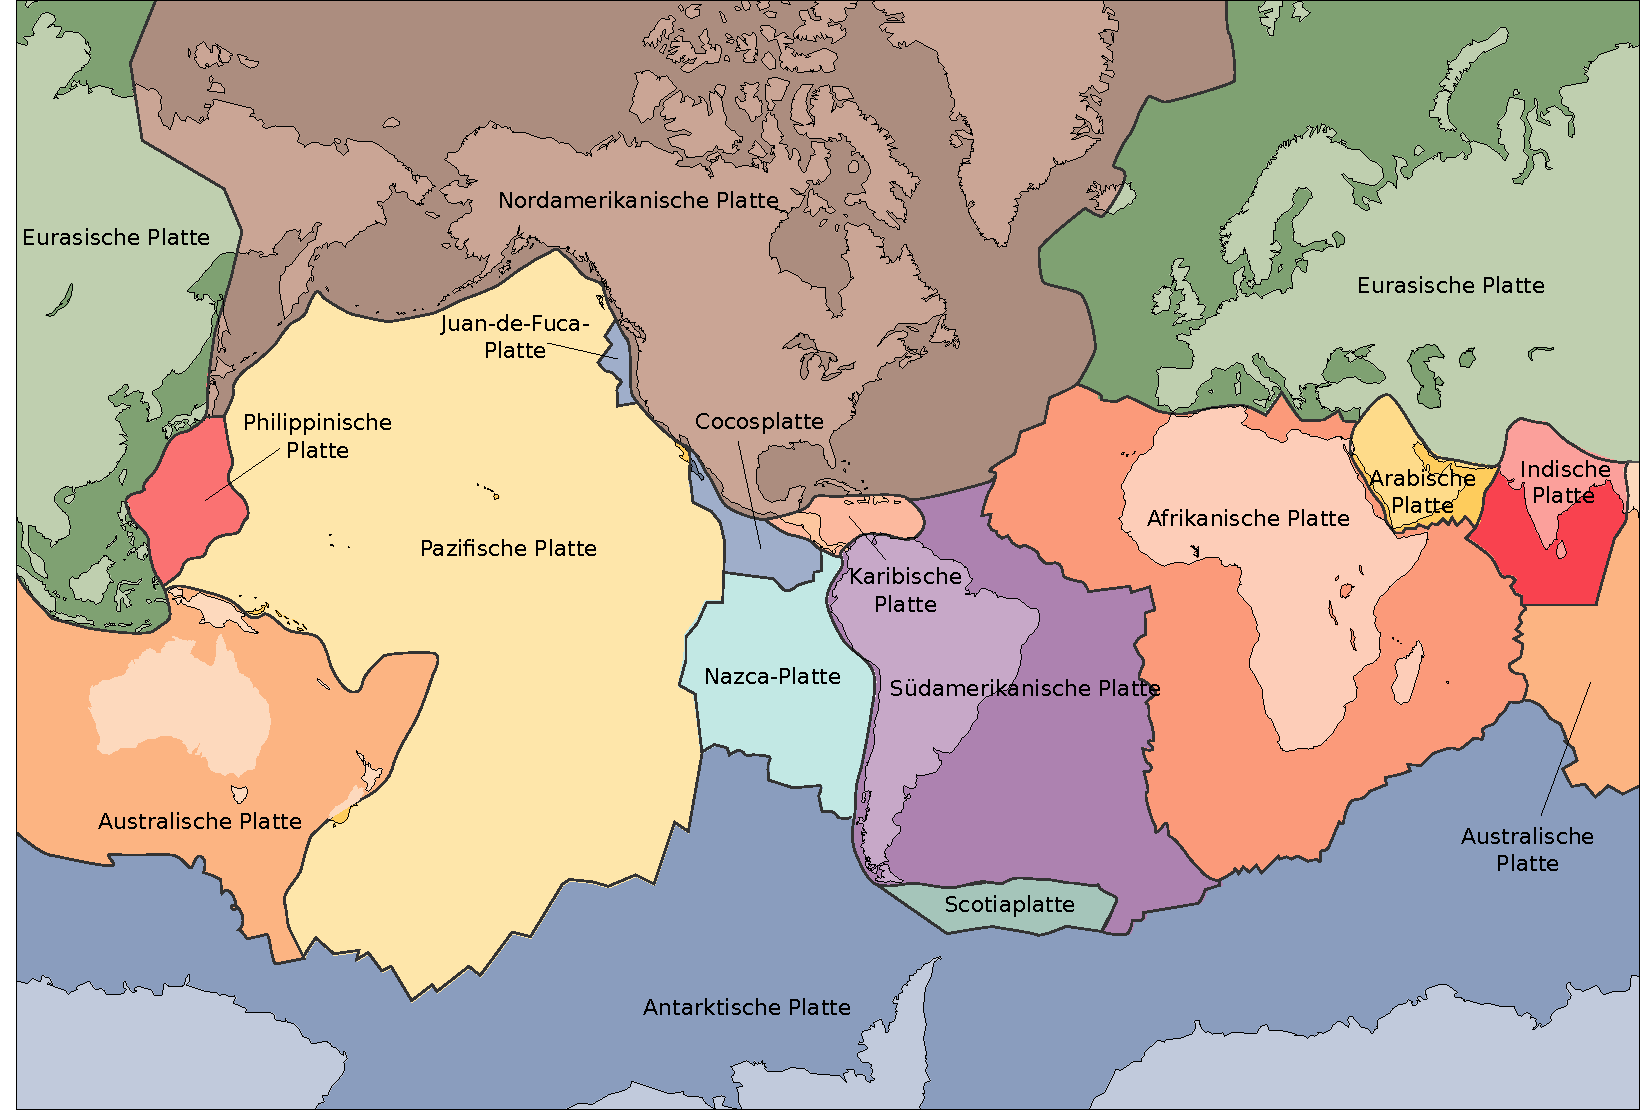
\includegraphics[width=0.75\linewidth]{%
        bilder/Tectonic_plates_de.pdf}
		\caption{Die Kontinentalplatten der Lithosphäre, Quelle: nach USGS.}
	\end{figure}

	\note{
		\begin{itemize}
			\item[] Die Lithosphäre wird in die Kontinentalplatten unterteilt, die sich in ständiger (sehr langsamer) Bewegung befinden (etwa \SI{10}{cm} pro Jahr).
			\item[$\rightarrow$] Durch aufeinander zudriftende Platten entstehen Gebirge (Himalaya, Alpen)
			\item[$\rightarrow$] Durch untereinander driftende Platten entstehen vulkanisch aktive Gebirgszüge (japanische Inseln, Anden)
			\item[$\rightarrow$] Durch voneinander weg driftende Platten entsteht der mittelozeanische Rücken
			\item[] Die ozeanische Erdkruste ist aufgrund der Subduktion (untereinander driften) in der Regel nur 160 bis 190 Millionen Jahre alt.
			\item[] Es gibt kontinentale Erdkruste, die bis zu 4 Milliarden Jahre alt ist.
			\item[] Die Lithosphäre wird durch Witterung zersetzt und Böden werden gebildet ($\rightarrow$ Pedosphäre)
		\end{itemize}
	}
\end{frame}
